\documentclass[10pt,conference,a4paper]{IEEEtran}
\usepackage[utf8]{inputenc}
\usepackage[T1]{fontenc}
% Correct date format in references but with american hyphenation, quotes, ...
% Trick from http://tex.stackexchange.com/a/129209
\usepackage[australian,american]{babel}

% *** GRAPHICS RELATED PACKAGES ***
\ifCLASSINFOpdf
  \usepackage[pdftex]{graphicx}
\else
  \usepackage[dvips]{graphicx}
\fi

% *** MATH PACKAGES ***
\usepackage{amssymb}
\usepackage[cmex10]{amsmath}

% Figure captions in small font
\makeatletter
\let\MYcaption\@makecaption
\makeatother
\usepackage[font=footnotesize]{subcaption}
\makeatletter
\let\@makecaption\MYcaption
\makeatother

\usepackage{pgfplots}
\pgfplotsset{compat=1.9}
%TODO minted ?
\usepackage[binary-units]{siunitx}
\usepackage{booktabs}
\usepackage{pifont}
\usepackage{tikz}
\usepackage{csquotes}
\usepackage[backend=biber,style=ieee,minbibnames=1,maxbibnames=3]{biblatex}
\usepackage{url}
%\usepackage[backgroundcolor=lightgray]{todonotes}
\usepackage[hidelinks]{hyperref}

\addbibresource{•}{paper.bib}
% Small font for references
\renewcommand*{\bibfont}{\small}

% correct bad hyphenation here
\hyphenation{op-tical net-works semi-conduc-tor}

% paper title
% can use linebreaks \\ within to get better formatting as desired
\def\mytitle{EpTO: An Epidemic Total Order Algorithm for Large-Scale Distributed Systems}
\title{\mytitle}

% author names and affiliations
% use a multiple column layout for up to three different
% affiliations
\def\jocelyn{Jocelyn Thode}
\def\ehsan{Ehsan Farhadi}
\author{\IEEEauthorblockN{\jocelyn\IEEEauthorrefmark{1},
\ehsan\IEEEauthorrefmark{2}}
\IEEEauthorblockA{Université de Neuchâtel\\
Neuchâtel, Switzerland\\
Email: \IEEEauthorrefmark{1}\href{mailto:jocelyn.thode@unifr.ch}{jocelyn.thode@unifr.ch},
\IEEEauthorrefmark{2}\href{mailto:ehsan.farhadi@unine.ch}{ehsan.farhadi@unine.ch}}}

% Set PDF file properties
\hypersetup{
	pdftitle=\mytitle,
}

% Tick marks
\newcommand{\cmark}{\ding{51}}
\newcommand{\xmark}{\ding{55}}

% Columns balancing
\renewbibmacro{finentry}{%
  \iffieldequalstr{entrykey}{jujjuri2010virtfs}%<- key after which you want the break
   {\finentry\newpage}
   {\finentry}}

\begin{document}
\graphicspath{{figures/}}


% make the title area
\maketitle


\begin{abstract}
One of the fundamental problems of distributed computing, is the ordering of events through all peers. From all the available orderings, total ordering is of particular interest as it provides a powerful abstraction for building reliable distributed applications. unfortunately, existing algorithms can not provide reliability, scalability, resiliency and total ordering in one package.	 EpTO is a total order algorithm with probabilistic agreement that scales both in the number of processes and events. EpTO provides deterministic safety and probabilistic liveness: integrity, total order and validity are always preserved, while agreement is achieved with arbitrarily high probability. We are going to implement EpTO using NeEM library and show EpTO is well-suited for large-scale dynamic distributed systems, and afterwards we will evaluate this algorithm by comparing it with currently being used ordering algorithms.
\end{abstract}

\section{Introduction}
%TODO
The ordering of events is one of the most fundamental problems in distributed systems, and it has been studied over past few decades. A lot of researchers have been working on an algorithm with different guarantees and tradeoffs such as synchronization, agreement or state machine replication. But because these properties are strong guarantees, the algorithms that implements them do not scale very well. Existing probabilistic protocols are highly scalable and resilient, but they can not provide total ordering in large scale distributed systems, and existing deterministic protocols which provide total ordering, are not resilient and scalable.
\par
The problem with current deterministic total ordering protocols, deterministic total ordering algorithm, is that they need some sort of agreement between all peers in the system. An agreement on the order of messages, which cause a massive amount of network traffic and overhead on the system.
Plus, an agreement feature for an asynchronous system requires to
explicitly maintain a group and have access to a failure detector. Due to the faults and churn in large-scale distributed systems, failure detector turns into bottleneck of the system and thus, limits scalability of the algorithm.
\subsection{Contribution}
EpTO guarantees that processes eventually agree on the set of received events with high probability and deliver these events in total order to the application. The intuition behind EpTO is that events are available quickly at all nodes with high probability,
Once events are thought to be available in every peer, each peer deterministically order them by timestamp of each event and breaking ties with the id of the broadcaster peer, and deliver them to the application accordingly.
\par
The main insight behind EpTO dissemination protocol is a \textit{balls-and-bins} approach. \textit{Balls-and-bins} is a basic probabilistic problem: consider \textit{n} balls and \textit{m} bins where we consequently throw balls into a bin, completely random and independent from other balls.
\par
A balls-and-bins approach abstract peers as bins and messages (events) as balls, and studies how many balls need to be \textit{thrown} such that each bin contains at least one ball with arbitrarily high probability. using this approach The number of messages transmitted per process per round is logarithmic in the number of processes, and the total number of messages
transmitted in the network before an event is delivered is low and uniform over all peers.

\begin{figure}
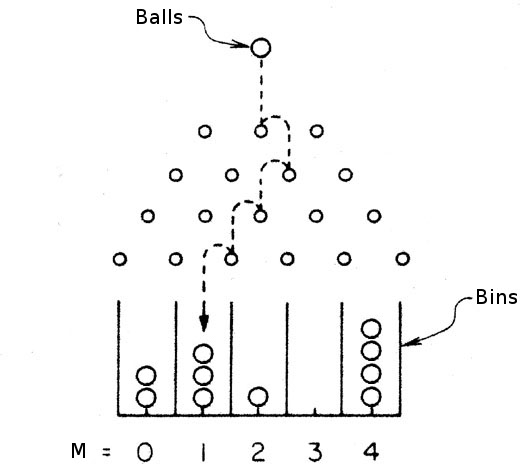
\includegraphics[width=\linewidth]{figures/BnB.jpeg}
\caption{balls-and-bins\protect\footnotemark{}.}
\label{fig:balls-and-bins}
\end{figure}

\section{EPTO ALGORITHM DESCRIPTION}
\subsubsection{EpTO Dissemination Component}
\subsubsection{EpTO Ordering Component}
\subsubsection{EpTO Stability Oracle}
\section{TODO}
\section{Work Plan}
\begin{figure}
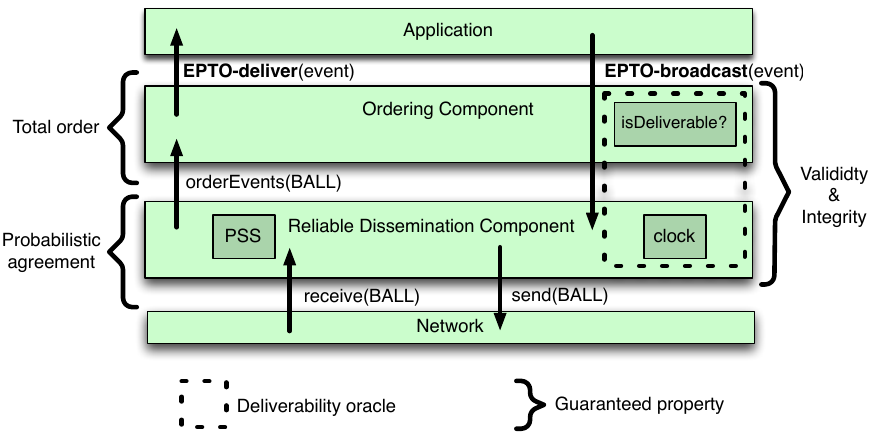
\includegraphics[width=\linewidth]{figures/epto-architecture.png}
\caption{test\protect\footnotemark{}.}
\label{fig:test}
\end{figure}





\section{Conclusion}
%TODO


% conference papers do not normally have an appendix


% use section* for acknowledgement
\section*{Acknowledgment}





% references section, with correct date format
\begin{otherlanguage}{australian}
\printbibliography
\end{otherlanguage}

% that's all folks
\end{document}
